\documentclass[letterpaper,12pt]{article}
\usepackage{amsmath}
\usepackage{amssymb}
\usepackage{amsthm}
\usepackage{graphicx}
%\usepackage{subfig}
\usepackage[margin=2.5cm,nohead]{geometry}

%\input{../commands}
%\setkeys{Gin}{draft=true}
%
%\newtheorem{thm}{Theorem}%[subsection]
%\newtheorem{lem}[thm]{Lemma}
%\newtheorem{cor}[thm]{Corollary}
%\newtheorem{prop}[thm]{Proposition}
%\newtheorem{remark}[thm]{Remark}
%\newtheorem*{thm*}{Theorem}
%\newtheorem*{lem*}{Lemma}



\begin{document}

\begin{center}
    {\bf UNIVERSITY OF CALIFORNIA AT BERKELEY}\\
    {\bf Department of Mechanical Engineering}\\
    {\bf ME233 Advanced Control Systems II}\\
    Spring 2012\\
\end{center}
\noindent
{\Large \bf Homework \#9 }\\[-3em]
\begin{flushright}
\begin{tabular} {lll}
    Assigned: &  Apr.\ 19 & (Th) \\
    Due: & Apr.\ 26 & (Th)
\end{tabular}
\end{flushright}

\begin{enumerate}

\item
Let $N_1$ and $N_2$ be two P-class nonlinearities:
\begin{align*}
    y_1(k) & = N_1(u_1(k))\\
    y_2(k) & = N_2(u_2(k))
\end{align*}
such that each satisfies the Popov inequality, i.e.
\begin{align*}
    \sum_{j=0}^k y_1^T(j)u_1(j) & \geq - \gamma_1^2
        & \sum_{j=0}^k y_2^T(j)u_2(j) & \geq  - \gamma_2^2
\end{align*}
Prove the following two propositions:
\begin{description}
    \item[Proposition 1:]
    The parallel combination of $N_1$ and $N_2$,
    \begin{align*}
    y(k) = N_1(u(k)) + N_2(u(k))
    \end{align*}
    satisfies the Popov inequality
    \begin{equation}
        \label{eq:Pine}
        \sum_{j=0}^k y^T(j)u(j)  \ge  - \gamma^2
    \end{equation}
    for some $\gamma \in \mathcal{R}$.

    \item[Proposition 2:]
    The negative feedback combination  of $N_1$ and $N_2$,
    \begin{align*}
        y(k) & = N_1(u(k) - y_1(k))\\
        y_1(k) & = N_2(y(k))
    \end{align*}
    satisfies the Popov inequality \eqref{eq:Pine} for some $\gamma \in \mathcal{R}$.
\end{description} 
\item
Consider the transfer function
\begin{align*}
    G(z) = \frac{z - b}{z - a}
\end{align*}
where $a,b \in \mathcal{R}$ and $|a| \neq 1$.

\begin{enumerate}
    \item
    Show that the frequency response of $G(z)$ touches the imaginary axis if and only if $\frac{b^2 - 1}{1 - a^2} \geq 0$.

%    \textbf{Hint:} First show that the frequency response of $G(z)$ touches the imaginary axis if and only if there exist $\omega \in [0,\pi]$ and $\beta \in \mathcal{R}$ such that
%    \begin{align*}
%        e^{j\omega} = \frac{b - j\beta a}{1 - j\beta} \; .
%    \end{align*}
%    Eliminate $\omega$ from this condition and then eliminate $\beta$ from the resulting condition.

    \item
    Find necessary and sufficient conditions on $a$ and $b$ for $G(z)$ to be strictly positive real.
\end{enumerate}

\newpage
\item
In this problem, you will conduct a simulation study of the series-parallel  identification algorithm that has been discussed in class. To this end, use the MATLAB file {\tt sp$\_$predict.m}, which is posted on bSpace.

The system that we want to identify is the second-order system given by
\begin{align*}
    y(k) = \frac{b_1q^{-1} + b_2 q^{-2}}{1 + a_1 q^{-1} + a_2 q^{-2}}\, u(k) + w(k)
\end{align*}
where $u(k)$ is the input and $w(k)$ is the measurement noise.
The PAA uses a series-parallel model and is governed by the equations
\begin{align*}
    e^o(k+1) & =  y(k+1) - \hat{\theta}^T(k) \, \phi(k) \\
    \phi(k) & = \begin{bmatrix}
            -y(k) & -y(k-1) & u(k) & u(k-1)
        \end{bmatrix}^T \\
    \hat{\theta}(k+1) & = \hat{\theta}(k) 
        + \frac{1}{\lambda_1(k) + \phi^T(k) F(k) \phi(k)} F(k) \phi(k)\,e^0(k+1) \\
    F(k+1) & = \frac{1}{\lambda_1(k)} \, \left[ F(k) - \lambda_2(k) 
        \frac{ F(k)\phi(k)\phi^T(k)F(k) }{ \lambda_1(k) + \lambda_2(k) \phi^T(k)F(k) \phi(k) } \right] \;
\end{align*}
The plant parameters are $a_1 = 1.7$, $a_2 = 0.72$, $b_1 =0.1$ and $b_2=0.05$. (Note that $A(q^{-1})$ is anti-Schur.)

Do the following and write a summary of your findings:
\begin{itemize}
    \item
    Try the least squares adaptation gain, least square adaptation  gains with a forgetting factor, and constant adaptation gains. For the cases when you are testing constant diagonal adaptation gains
    $F = {\rm Diag}(F_{11},\,F_{22},\,F_{33},\,F_{44})$, analyze the effect on the parameter convergence of the relative magnitude between  the submatrices ${\rm Diag}(F_{11},\,F_{22})$ and ${\rm Diag}(F_{33},\,F_{44}$).  Try ratios such as 1/100, 1/10, 1/1, 10/1, etc.

    \textbf{Note:} When the adaptation gain is constant, the correction terms for $a_i$'s are proportional to  ${\rm Diag}(F_{11},\,F_{22}) \times y$, while those for the $b_i$'s are proportional to  ${\rm Diag}(F_{33},\,F_{44}) \times u$. You should see that balanced, and hence faster, convergence takes place when all correction terms are more or less of the same size.

    \item
    Verify the effect of the persistence of excitation (or lack thereof) of the input sequence $u(k)$ on the parameter error convergence.

    \item
    Check what the effect of white measurement noise $w(k)$ is on the parameter error convergence (i.e.\ turn  the noise term on and off).
\end{itemize}

\newpage
\item
In this problem, you will conduct the stability analysis of a parallel  PAA identification algorithm. The system that we want to identify is the second-order system given by
\begin{align*}
    y(k) = \frac{b_1q^{-1} + b_2 q^{-2}}{1 + a_1 q^{-1} + a_2 q^{-2}} u(k) \; .
\end{align*}
Note that the system dynamics can be written as
\begin{align*}
    y(k+1) & = \theta^T \phi(k) \\
    \phi(k) & = \begin{bmatrix}
            -y(k) & -y(k-1) & u(k) & u(k-1)
        \end{bmatrix}^T \\
    \theta & = \begin{bmatrix}
            a_1 & a_2 & b_1 & b_2
        \end{bmatrix}^T \; .
\end{align*}
The PAA uses a parallel model and is governed by the equations
\begin{align}
    \hat{\phi}(k) & = \begin{bmatrix}
            -\hat{y}(k) & -\hat{y}(k-1) & u(k) & u(k-1)
        \end{bmatrix}^T
        \label{eq:parallel_PAA_first} \\
    \hat{y}^o(k+1) & = \hat{\theta}^T(k) \, \hat{\phi}(k) \\
    e^o(k+1) & =  y(k+1) - \hat{y}^o(k+1) \\
    v^o(k+1) & = e^o(k+1) + c_1 \, e(k) + c_2 \, e(k-1) \\
    v(k+1) & = \frac{ \lambda_1(k) }{ \lambda_1(k) + \hat{\phi}^T(k) F(k) \hat{\phi}(k) } v^o(k+1) \\    \hat{\theta}(k+1) & = \hat{\theta}(k) + \frac{1}{\lambda_1(k)} F(k) \hat{\phi}(k)\,v(k+1) \\
    \hat{y} (k+1) & = \hat{\theta}^T(k+1) \hat{\phi}(k) \\
    e(k+1) & = y(k+1) - \hat{y}(k+1) \\
    F(k+1) & = \frac{1}{\lambda_1(k)} \, \left[ F(k) - \lambda_2(k)
        \frac{ F(k) \hat{\phi}(k) \hat{\phi}^T(k)F(k) }
        { \lambda_1(k) + \lambda_2(k) \hat{\phi}^T(k)F(k) \hat{\phi}(k) } \right]
        \label{eq:parallel_PAA_last}
\end{align}
where $0 < \lambda_1(k) \leq 1$, $0 \leq \lambda_2(k) < 2$ and the constants $c_1$ and $c_2$ must be selected so that the transfer function
\begin{align}
    \label{eq:gq}
    G(z^{-1}) = \frac{1 + c_1 \, z^{-1} + c_2\, z^{-2}}{ 1 + a_1 \, z^{-1} + a_2\, z^{-2}}
\end{align}
has the necessary properties. (You will determine what these properties are.)

\begin{enumerate}
    \item
    Show that $v(k+1) = e(k+1) + c_1 e(k) + c_2 e(k-1)$.

    \item
    Using the result of the previous part, show that the relationship
    \begin{equation}
    \begin{aligned}
        v(k) & = G(q^{-1}) m(k) \\
        m(k) & = \tilde{\theta}^T(k) \hat{\phi}(k-1)
    \end{aligned} \label{eq:efl}
    \end{equation}
    holds, where $G(z^{-1})$ is given by Eq. \eqref{eq:gq}, and $\tilde{\theta}(k) = \theta - \hat{\theta}(k)$.

    \textbf{Hint:} As the first step in the proof, use the expressions for $y(k+1)$ and $\hat{y}(k+1)$ to show that
    \begin{align}
        e(k+1) = - a_1 e(k) - a_2 e(k - 1) + m(k+1) \; .
        \label{eq:ek_mk}
    \end{align}
    Then use the result of part (a) to complete the problem.

    \item
    Using the results of the previous part, the PAA error dynamics can be represented by the block diagram in Fig.~\ref{fig:hyperstability_basic_block}.
    \begin{figure}[h]
        \centering
        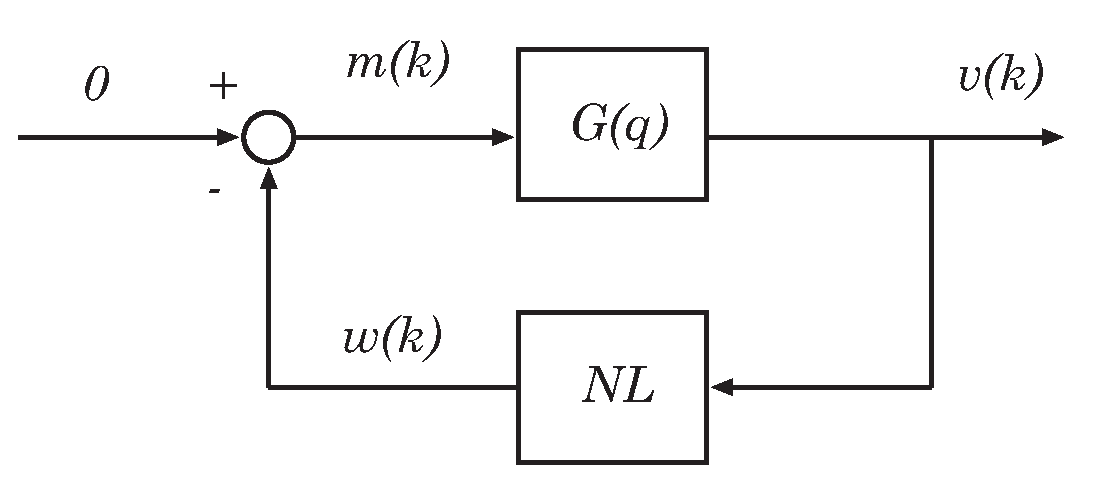
\includegraphics[width=6cm]{hyperstability_basic_block}
        \caption{Parallel PAA error dynamics}
        \label{fig:hyperstability_basic_block}
    \end{figure}
    Perform the same series of block diagram operations to the block diagram in Fig.~\ref{fig:hyperstability_basic_block} as were performed in Lecture 21 on slides 26--31. The resulting equivalent feedback loop should have an LTI system in negative feedback with a \underline{P-class} nonlinear block.

    \item
    State the properties that $G(z^{-1})$ must satisfy in order to use the asymptotic hyperstability theorem to prove asymptotic hyperstability of the equivalent feedback loop determined in part (c).

    \item
    Under the conditions determined in the previous part, show that $e^o(k)$, $e(k)$, $v^o(k)$, and $v(k)$ converge to zero. Assume that $u(k)$ and $F(k)$ are bounded.
\end{enumerate} 
\newpage
\item
In problem 3, you conducted a simulation study of the series-parallel identification algorithm that has been discussed in class. In this problem you are asked to conduct a similar simulation study of the parallel identification algorithm that you analyzed in problem 4.

The system that we want to identify is the same as the one in problem 3, i.e.
\begin{align*}
    y(k) = \frac{b_1q^{-1} + b_2 q^{-2}}{1 + a_1 q^{-1} + a_2 q^{-2}}\, u(k) + w(k)
\end{align*}
where $u(k)$ is the input and $w(k)$ is measurement noise. The plant parameters are $a_1 = 1.7$, $a_2 = 0.72$, $b_1 =0.1$ and $b_2=0.05$.

\begin{enumerate}
    \item
    Select $\bar{\lambda} \leq 1$ and a set of constants $c_1$ and $c_2$ so that:
    \begin{itemize}
        \item $c_i \neq a_i$, $i=1,2$ and
        \item $G(z^{-1})$ in \eqref{eq:gq} satisfies the conditions that you determined in problem 2(c).
    \end{itemize}

    \item
    Using the matlab file {\tt sp$\_$predict.m} as your starting point, create a MATLAB file
    %{\tt p$\_$predict$\_${\em your-last-name}.m}
    that implements the parallel RLS PAA in Eqs.~\eqref{eq:parallel_PAA_first}--\eqref{eq:parallel_PAA_last}. Compare the parameter convergence of the parallel algorithm with that of the series-parallel algorithm, using similar initial conditions, under the following cases:
    \begin{enumerate}
        \item
        Random input $u(k)$, no measurement noise, and least square gain (without forgetting factor).

        \item
        Random input $u(k)$, no measurement noise, and least square gain with forgetting factor.
        \item
        Random input $u(k)$, white measurement noise, and least square gain (without forgetting factor).

        \item
        Random input $u(k)$, colored measurement noise, and least square gain (without forgetting factor).
    \end{enumerate}
    Write a short summary of your findings. (You do not need to submit your modified version of {\tt sp$\_$predict.m})

%    \textbf{Note:} To perform the simulations for the parallel RLS PAA, it will be easiest to create a new function based on {\texttt sp$\_$predict.m}.
\end{enumerate}




\end{enumerate}


\end{document}


